\documentclass[aspectratio=169,hyperref={pdfpagelabels=false}]{beamer}
\usepackage{helvet}
\usepackage[english]{babel}
\usepackage{pgfplots}
\usepackage{pgf}
\pgfplotsset{compat=newest}
\usepackage{booktabs}
\usepackage[T1]{fontenc}
\usepackage[utf8]{inputenc}
\usepackage{lipsum}
\usepackage{tcolorbox}
\usepackage{xcolor}
\usepackage{listings}
\usepackage{microtype}
\usepackage{float}
\usepackage{siunitx}
\usepackage{multicol}
\usepackage{hyperref}
\usepackage{dsfont}
\usepackage{caption}
\usepackage{subcaption}

\input{template/settings}

\newcommand{\setcolor}[1]{\def\chosencolor{#1}}
\newcommand{\setdepartment}[1]{\def\department{#1}}

\usetheme{DTU}
\setbeamersize{text margin left=22mm}
\def\insertframetitle{}

\newcommand{\inserttitlepage}{

    \begin{frame}[plain]{}
        \color{white}\maketitle    
    \end{frame}

    \setbeamercolor{background canvas}{bg = white}
}

\subtitle{Project in 31011 Engineering Practices}
\title{Error Correction in Digital Systems}
\author{Tjark Petersen}
\setcolor{orange}

\usepackage{multicol}
\usepackage{hyperref}
\usepackage{siunitx}
\usepackage{biblatex}

\addbibresource{ref.bib}

\newcommand{\sectionseperator}[1]{%

{%
\setbeamercolor{background canvas}{bg=\chosencolor}
\begin{frame}[plain]{}

        \usebeamercolor[fg]{title}

        \begin{center}
        \hspace{-3.6em}\vspace{-3.6em}{\usebeamerfont{title}\textbf{#1}\par}
        \end{center}

        
\end{frame}
}

}


\begin{document}
\inserttitlepage

\begin{frame}{Outline}

    \begin{itemize}
        \item Theoretical background
        \item Fundamental principles of error correction
        \item Error correction codes
        \item The project
    \end{itemize}

\end{frame}

\begin{frame}{About me}
    \begin{columns}


        \begin{column}{0.2\textwidth}
        \begin{figure}
            \centering
            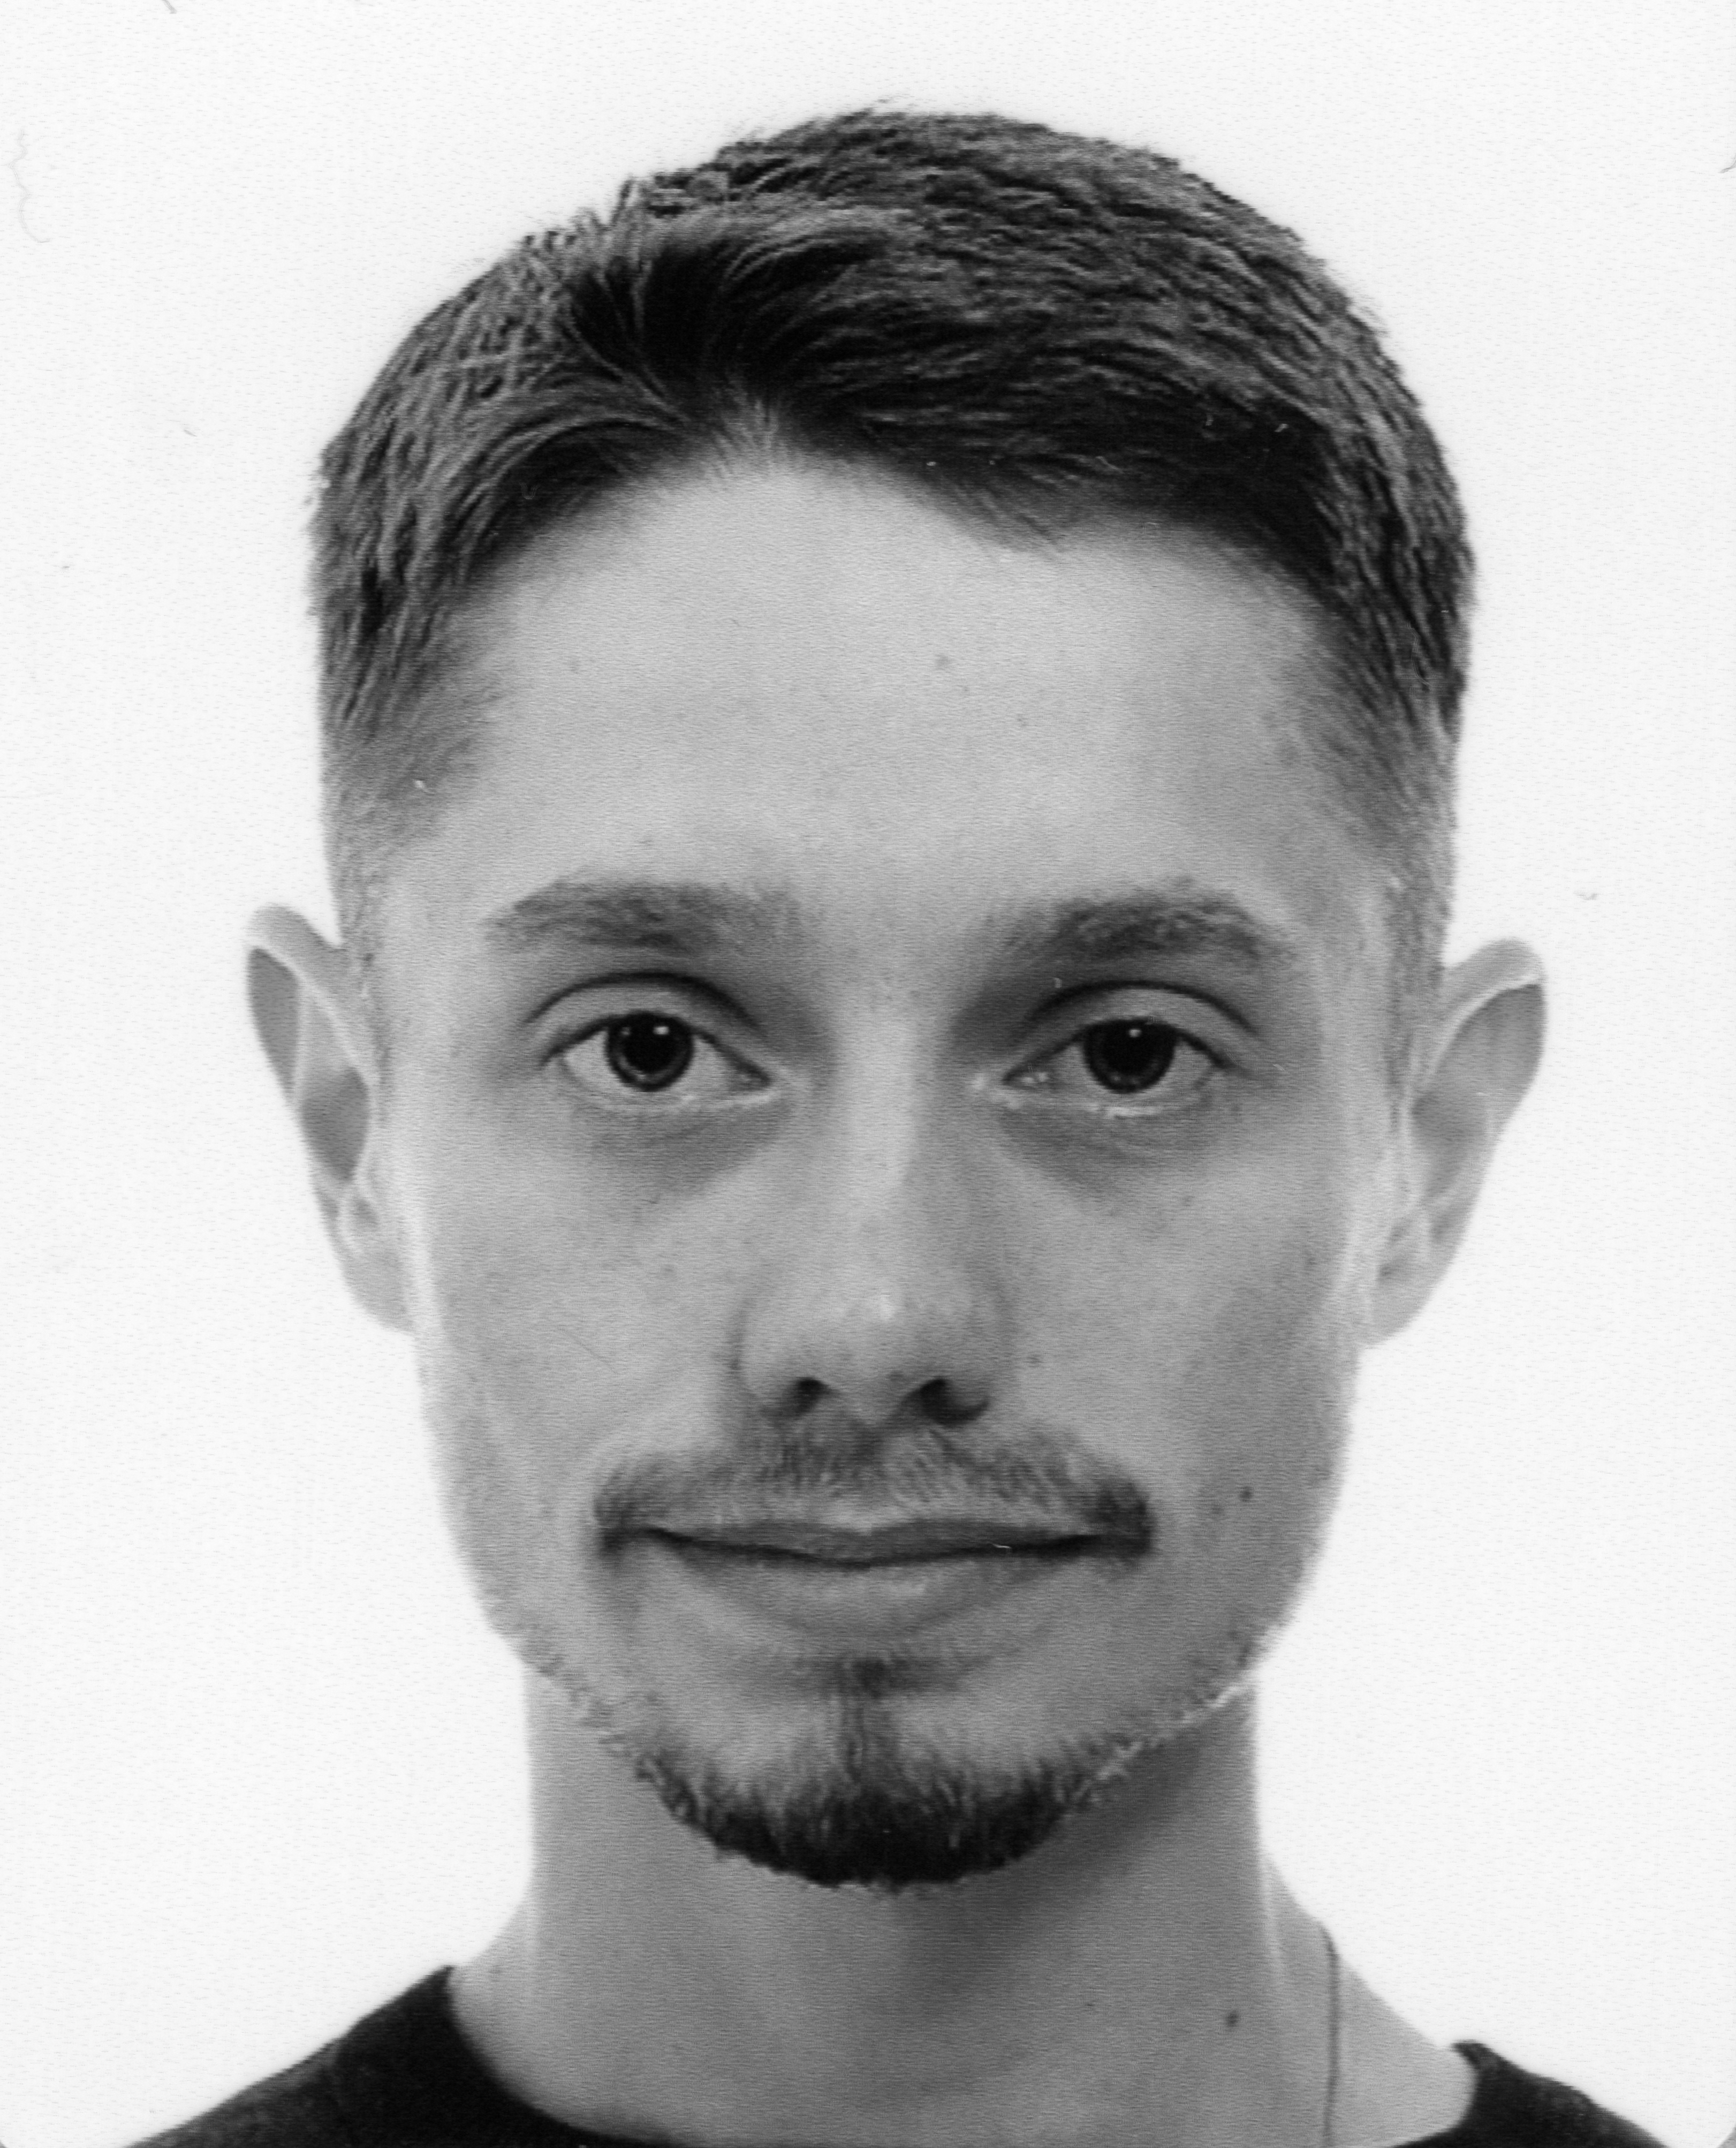
\includegraphics[width=2cm]{fig/pass2020.png}
        \end{figure}
        \end{column}
        
        \begin{column}{0.8\textwidth}
        \begin{itemize}
            \item Tjark Petersen (tjape@dtu.dk)
            \item From Germany but living in Denmark since 2017
            \item BSc. in Electrical Engineering here at DTU
            \item Now enrolled in MSc. in Computer Science and Engineering
            \item Interested in computer architecture, digital systems and embedded systems
        \end{itemize}
        \end{column}
        
        \end{columns}
\end{frame}

\sectionseperator{Theoretical Background}

\begin{frame}{The Fundamental Problem}
    % noisy channel
    \begin{itemize}
        \item Information is sent from $X$ to $Y$ via a \textit{noisy channel}
        \item The noisy channel randomly induces bit flips in the transmitted piece of information
        \item Therefore $X\neq Y$
    \end{itemize}
    \begin{figure}
        \includegraphics[width=8cm]{fig/NoisyChannel.pdf}
    \end{figure}
\end{frame}

\begin{frame}{In Transmission Systems}
    % electric interference
    \begin{multicols*}{2}
        \begin{itemize}
            \item Channel is a wire
            \item Noise could originate from:
            \begin{itemize}
                \item Power supply
                \item Other circuit components via the power network
                \item Other nearby wires via inductive coupling
            \end{itemize}
            \item Digital signals are very resilient with respect to noise
        \end{itemize}

        \begin{figure}
            
            \includegraphics[width=4cm]{fig/Digital-signal-noise.png}
            \caption{A noisy digital signal\footnotemark}
        \end{figure}
    \end{multicols*}

    \footnotetext{\tiny{\url{https://en.wikipedia.org/wiki/Digital\_signal\#/media/File:Digital-signal-noise.svg}}}
  
\end{frame}

\begin{frame}{In Memory Systems}

    \begin{columns}

        \begin{column}{0.56\textwidth}
            \begin{itemize}
                \item Channel \textit{stores} information such that it can be retrieved at another point in time
                \item Memory is organized into $n$ addresses which each can hold $w$ bits of data 
                \item Hard errors result in a memory cell being stuck at a constant value
                \item Soft errors leave the affected memory cells intact but flip the stored bit
            \end{itemize}
        \end{column}
        
        \begin{column}{0.39\textwidth}
            \begin{figure}
                \includegraphics[width=6cm]{fig/Memory.pdf}
            \end{figure}
        \end{column}
        

        
    \end{columns}
    % cosmic particles
    % DRAM
    % SRAM
    % show common FIT
\end{frame}

\begin{frame}{Dynamic Random-Access Memory}
    
    \begin{columns}
        \begin{column}{0.56\textwidth}
            \begin{itemize}
                \item A capacitor is charged (1) or uncharged (0) through a transistor
                \item The transistor is turned off and the capacitor holds its charge
                \item When the transistor is turned on again, the stored bit can be observed on the data line
                \item Capacitors leak (hence \textit{dynamic}) and memory cells need to be refreshed with an interval in the range of milliseconds in modern DRAM
            \end{itemize}
        \end{column}
        \begin{column}{0.39\textwidth}
            \begin{figure}
                \includegraphics[width=4cm]{fig/dram_cell.pdf}
                \caption{A DRAM cell}
            \end{figure}
        \end{column}
    \end{columns}

\end{frame}

\begin{frame}{Static Random-Access Memory}
    \begin{columns}
        \begin{column}{0.56\textwidth}
            \begin{itemize}
                \item Two cross-coupled inverters ($M_1$-$M_4$) + two access Transistors ($M_5$ and $M_6$)
                \item While powered, the two inverters have a stable 0 and 1 state (hence \textit{static})
                \item Higher static power draw and lower density compared to DRAM
            \end{itemize}
        \end{column}
        \begin{column}{0.39\textwidth}
            \begin{figure}
                \includegraphics[width=5cm]{fig/SRAM_Cell_(6_Transistors).png}
                \caption{A 6 transistor SRAM cell\footnotemark}
            \end{figure}
        \end{column}
    \end{columns}
    \footnotetext{\tiny{\url{https://en.wikipedia.org/wiki/Static\_random-access\_memory\#/media/File:SRAM\_Cell\_(6\_Transistors).svg}}}
\end{frame}

\begin{frame}{Soft Error Sources}
    
    \begin{itemize}
        \item Charged particles can interact with capacitors or transistors and disrupt their state
        \item With smaller chip manufacturing process sizes ($\SI{5}{nm}$ today) the critical charge needed to tip the logic state of a circuit element shrinks
        \item Thermal neutrons can break a Silicon nucleus creating charged nuclei that interact with the circuit
        \item $\alpha$-particles from radioactive sources can interact with circuits elements through their charge
        \item High energy cosmic particles can interact with the circuit through their charge
    \end{itemize}

\end{frame}

\begin{frame}{How Often Do Soft Errors Occur?}

    \begin{itemize}
        \item Error rates are measured in failure-in-time (FIT) describing the number of failures in 1 billion device operation hours
        \item Older study found DRAM soft error rates of $\SI{1000}{FIT/MBit}$ \cite{soft_error_in_e_mem}
        \begin{itemize}
            \item Mean time between failure with $\SI{512}{MB}$ of memory: $10^9 / (1000\cdot (512\cdot8)) \approx \SI{244}{hours}$
        \end{itemize} 
        \item Large scale field study in Google data centers found 25,000 to 70,000 combined soft and hard errors per billion device hours per Mbit for DRAM system memory \cite{errors_in_wild}
        \item 1 megagate SRAM-based FPGA associated with ground-level soft error rate of $\SI{1200}{FITs}$ \cite{actel}
        \begin{itemize}
            \item System with 100 of these FPGAs would have a functional error every 11 months
        \end{itemize} 
    \end{itemize}
    
\end{frame}

\sectionseperator{Solutions}

\begin{frame}{Redundancy}
    \begin{itemize}
        \item If every bit that is sent holds a unique piece of information, its corruption means a direct loss of information
        \item We can encode information about the actual message in additional redundant bits which are sent together with the message
        \item Thus each message bit is no longer the only carrier of its piece of information, but that information is distributed over multiple bits
        \item The higher the level of redundancy, the more loss of information during transmission can be tolerated
    \end{itemize}
\end{frame}

\begin{frame}{Error Detection vs. Error Correction}

    \begin{itemize}
        \item Option 1:
        \begin{itemize}
            \item Give receiver the ability to detect that up to $n$ bits have been flipped and request a resend
        \end{itemize}
        \item Option 2:
        \begin{itemize}
            \item Give receiver the ability to detect and correct up to $m$ bits in a corrupted message
        \end{itemize}
        \item Option 3:
        \begin{itemize}
            \item Give receiver the ability to detect up to $n$ bit flips and correct up to $m$ of them with $n>m$ and only request a resend if more than $m$ bit flips occured
        \end{itemize}
        \item In all cases, if the number of bit flips exceeds the maximum number that can be detected, the information is seen as uncorrupted by the receiver
    \end{itemize}
    % long latency -> resend is costly
\end{frame}



\begin{frame}{Throughput vs. Resilience}
    % more redundancy -> can recover multiple errors -> fewer "real" bits sent
    \begin{itemize}
        \item The higher the number of bit flips to be detected/corrected, the more redundancy has to be added in the encoded message
        \item At a given transmission rate, with higher redundancy comes a loss of throughput of actually useful data
        \item With less redundancy, fewer errors can be tolerated
        \item A trade-off has to be made based on throughput requirements and expected error rates
    \end{itemize}
\end{frame}

\sectionseperator{Error Detection}

\begin{frame}{Even/Odd Parity}

    \begin{itemize}
        \item Very common and lightweight way to detect single bit errors
        \begin{itemize}
            \item For instance used in UART protocol
        \end{itemize}
        \item Add one additional bit to message, the parity bit
        \item Count 1s in message
        \item Even parity: Make the total number of 1s in the message even using the parity bit
        \item Odd parity: Make the total number of 1s in the message odd using the parity bit
        \item Example with even parity: $X=abcd=1101\Longrightarrow M=abcdp=11011$
    \end{itemize}
    
\end{frame}

\sectionseperator{Error Correction Codes}

\begin{frame}{Error Correction Codes}
    % send data which is function of real data with data
    \begin{itemize}
        \item Systematically use redundant bits to encode information about the message
        \item Use redundant bits to reconstruct original message
        \item $X_{\texttt{w-1:0}}\Longrightarrow M_{\texttt{w+r-1:0}}=enc(X) \Longrightarrow Y_{\texttt{w-1:0}}=dec(M)$
        \item $enc(A_{\texttt{w-1:0}})$ and $dec(B_{\texttt{w+r-1:0}})$ are functions defined by the error correction code
    \end{itemize}
    \begin{figure}
        \includegraphics[width=0.8\textwidth]{fig/NoisyChannel_plus_ecc.pdf}
    \end{figure}
\end{frame}

\begin{frame}{Block Codes vs. Continuous Codes}
    \begin{itemize}
        \item Error correction codes can be optimized for two different scenarios:
        \begin{itemize}
            \item A single message is sent every now and then
            \item A constant stream of data is sent
        \end{itemize}
        \item Block codes generate their redundant bits only based on the current message
        \item Continuous codes keep \textit{state} in between messages such that the redundant bits of a message depend on the current and previous messages
    \end{itemize}
\end{frame}

\begin{frame}{Majority Vote (Triple Modular Redundancy)}
    \begin{itemize}
        \item Simple scheme: Send three copies of each bit and let a majority vote decide on the bit value on the receiver end
        \item Example: $X=abc=010 \Longrightarrow M=aaabbbccc=000111000$
        \item If only one of our three copies of a bit changes per bit, we can recover the original message
        \item But our actual throughput is only 1/3 of what it could be!
        \item For storage systems we would have to store 3 times as much data!
        \item Can we do better?
    \end{itemize}
\end{frame}

\begin{frame}{Hamming code}
    
    \begin{itemize}
        \item Hamming developed a scheme which allows for the detection and localization of a single bit error 
        \item It uses \textit{parity} for localizing the error
        \item The equation $2^p \geq d+p+1$ ($d=\text{data-bits}$, $p=\text{parity-bits}$) tells us how many additional bits we need to add given a data bit-width
        \item A popular choice is the Hamming code (7,4) with 4 data-bits and 3 parity-bits
        
    \end{itemize}
        
    \end{frame}
    
    \begin{frame}{Hamming code (7,4)}
    
    \begin{columns}
    
    \begin{column}{0.6\textwidth}
    
    \begin{itemize}
        \item Group the 4 bits into 3 distinct groups of 3 bits and assign each group a parity bit
        \item Set the parity-bits such that the group and the parity bit together have even parity
        \item After a single error occurs, one or more groups will no longer have even parity
        \item Looking at which groups now have odd parity tells us which bit flipped unambiguously
    \end{itemize}
    
    \end{column}
    
    
    
    \begin{column}{0.4\textwidth}
    \vspace{-1cm}
    \begin{figure}
        \centering
        \includegraphics[width=4.8cm]{fig/hamming7_4.pdf}
    \end{figure}
    
    \begin{figure}
        \includegraphics[width=3.3cm]{fig/Hamming(7,4).png}
        \caption{See\footnotemark}
    \end{figure}
    
    
    \begin{center}
    \begin{tabular}{c}
    $0 = p_0 \oplus d_0 \oplus d_1 \oplus d_3$ \\
    $0 = p_1 \oplus d_0 \oplus d_2 \oplus d_3$ \\
    $0 = p_2 \oplus d_1 \oplus d_2 \oplus d_3$
    \end{tabular}
    \end{center}
    \end{column}
    
    \end{columns}

    \footnotetext{\tiny{\url{https://en.wikipedia.org/wiki/Hamming\_code\#/media/File:Hamming(7,4).svg}}}
        
    \end{frame}
    
    
    \begin{frame}{Hamming code (7,4) - Example}
    
    \begin{figure}
        \centering
        \includegraphics[width=11cm]{fig/Hamming7_4_example.pdf}
    \end{figure}
    
    \begin{center}
    \begin{tabular}{c}
    $ p_0 \oplus d_0 \oplus d_1 \oplus d_3 = 1 \oplus 1 \oplus 1 \oplus 1 = 0$ \\
    $p_1 \oplus d_0 \oplus d_2 \oplus d_3 = 0 \oplus 1 \oplus 1 \oplus 1 = 1$ \\
    $p_2 \oplus d_1 \oplus d_2 \oplus d_3 = 0 \oplus 1 \oplus 1 \oplus 1 = 1$
    \end{tabular}
    \end{center}
    Only $d_2$ could have changed the second and third equation while not changing the first equation. We can fix the error by inverting the third data bit.\\\vspace{0.4cm}
    If we concatenate the results of the 3 parity checks: $110_{two} = 6_{ten}$ we get the position of the error in the 1-indexed encoded message!
    
    \end{frame}


\begin{frame}{General Hamming Code}
    \begin{itemize}
        \item Other Hamming codes include: (15,11), (31,26), (63,57), (127,120) or (255,247)
        \item Rate of parity bits per data bits improves
        \item But chance of multiple bit flips in single hamming encoded message increases
    \end{itemize}
\end{frame}

\begin{frame}{Hamming SEC-DED}
    \begin{itemize}
        \item Popular option: Single Error Correction - Double Error Detection
        \item Add an additional parity bit that covers all parity and data bits
        \item If one error occurs, the overall parity changes
        \item If two errors occur, the overall parity stays the same
    \end{itemize}
\end{frame}

\begin{frame}{ECC in the real world}

    \begin{itemize}
        \item Servers often use ECC capable system memory built around Hamming codes
        \item Mass storage usually includes more advanced error correction schemes
        \item Many communication protocols include error detection capabilities:
        \begin{itemize}
            \item UART protocol has a parity bit
            \item Ethernet frames use cyclic redundancy checks
            \item IPv4 packets use checksums
        \end{itemize}
    \end{itemize}
    
\end{frame}

\sectionseperator{The Project}

\begin{frame}{Project Plan}

    \begin{itemize}
        \item Start with some exercises on Hamming code and literature review on soft errors
        \item Implement part of an error correction capabable system in VHDL
        \item Write a technical report covering the theoretical background and your implementation using LaTeX
    \end{itemize}

    \begin{figure}
        \includegraphics[width=\textwidth]{fig/CoursePlan.pdf}
    \end{figure}
    
\end{frame}

\begin{frame}{References}
    \printbibliography
\end{frame}


\end{document}